\documentclass{article}
% bibliography setup
\usepackage{natbib}
\bibliographystyle{apalike}  % abbrvnat
\setcitestyle{authoryear,open={(},close={)}} %Citation-related commands
% makes color citations
\usepackage[colorlinks=true,urlcolor=blue,citecolor=red,linkcolor=red,bookmarks=true]{hyperref}
% images
\usepackage{graphicx}
\graphicspath{ {./images/} }

% hypter parameter setup
\usepackage{hyperref}
% for table setup
\usepackage{tabularx}

\title{Improved Sequential Hypothesis Testing with
``Enhanced Precision Is The Goal"}
\date{\today}
\author{Eyal A. Kazin}

\begin{document}
\maketitle

\input precision_goal_abstract

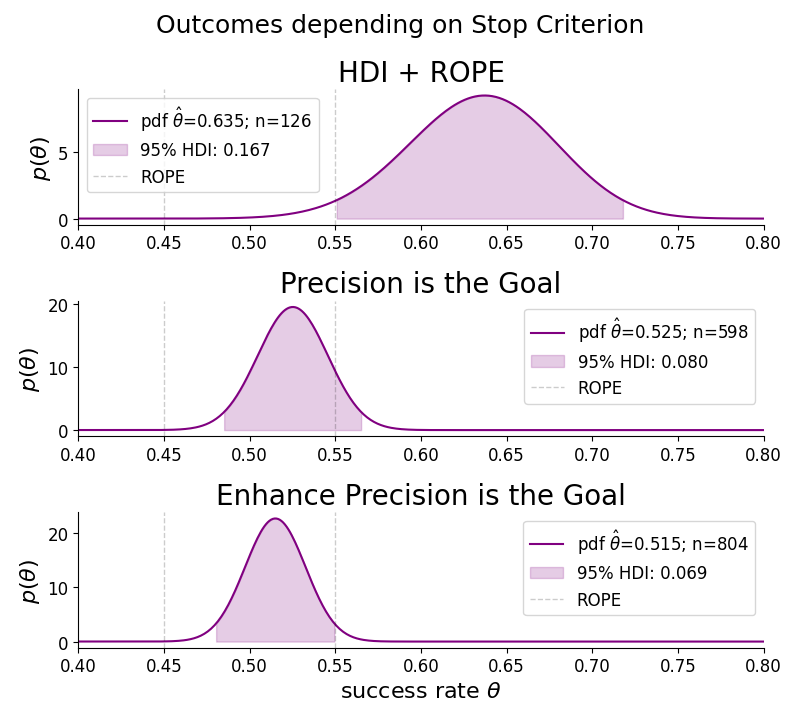
\includegraphics[scale=0.5]{cherry_posteriors.png}

%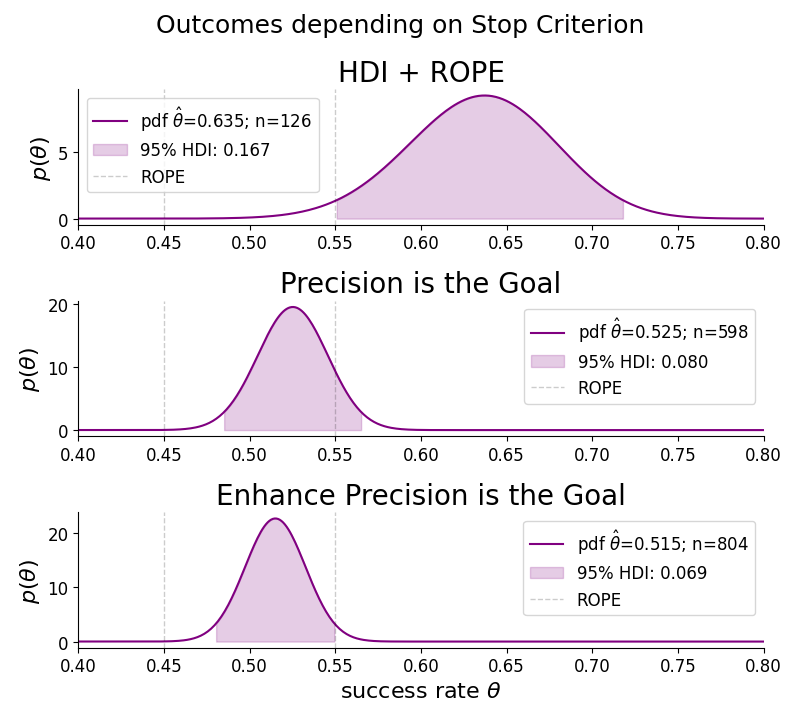
\includegraphics[width=1\textwidth]{cherry_posteriors.png}

\begin{figure}[h]
    \centering
    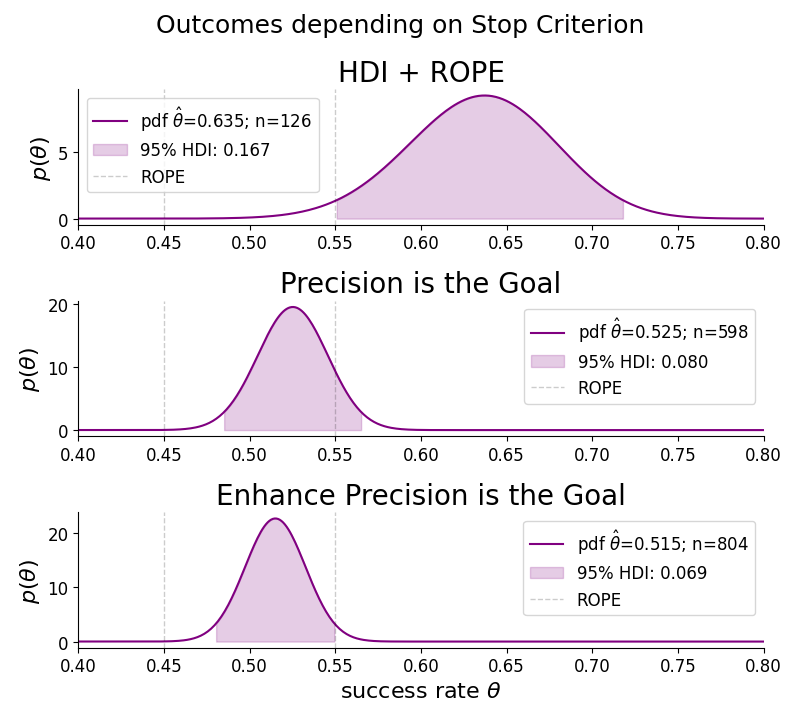
\includegraphics[width=1\textwidth]{cherry_posteriors.png}
    \caption{Beta function posteriors of subsamples of example sequence from Figure REF. Panels are results of different stop/decision criteria being triggered. Shaded areas are 95\% HDIs. ROPE within vertical dashed lines.
    Top - HDI+ ROPE triggers when the 95\% HDI is fully outside the ROPE (iteration 126). Incorrectly rejects $\theta_{\rm null}$. Middle - “Precision is the Goal” triggers when 95\% HDI width reaches precision goal of 80\% ROPE width (iteration 598). HDI straddles the ROPE → inconclusive.
    Bottom - “Enhanced Precision is the Goal” triggers when 95\% HDI fully within ROPE and obtains same precision goal (iteration 804). Correctly accepts $\theta_{\rm null}$}
\end{figure}

\section{Introduction}
\input precision_goal_introduction

\subsection{Contributions}

\subsubsection{Paper Structure}
The paper is organized as follows.
In the Methods section we describe three (four if Frequentist?)
stop criteria as well as the setup to test on synthetic deichotomous data.
In the Results section we present the results of the synthetic data analysis as well as analytical analysis.
In the Discussion section we discuss the implications of the results (Reword this).
In the Conclusion section we summarize the findings and suggest future directions (Reword this).


\section{Methods}

Here we describe three stop criteria for sequential hypothesis testing,
all of which rely on the same decision criterion to determine acceptence
or rejection of the null hypothesis.

We describe and contrast the algorithms intuitively, as well as in pseudo code.
We provide also anlaytical useful experessions and conclude by describing a setup
to test the methods on synthetic dichotomous data.
Although our belief is that these methods apply to any type of data,
our focus is on Bernouli trials in order to compare with \cite{kruschke2015doing}
(somehow experess that: "as it is simple to describe analytically and
to conduct rapid tests on synthetic data.")

\subsection{One Decision Criterion And Three Stop Criteria}

Table (cite table) provides an intuitive comparison between the three algorithms of interst.
In order to conduct this comparison we consider:
\begin{itemize}
    \item Pre Survey Decisions - the parameters required to decide ahead of data
    collection
    \item The stop criterion main characteristic 
    \item The decision criterion characteristic
    \item Stop and Decision order - are they simultaneous a two step process?
\end{itemize}
By creterion {\it characteristic} we are referring to the property of the posterior of
importance: its location and/or width

% make a table in latex with four rows and 5 columns

\begin{tabularx}{1.2\textwidth} { 
    | >{\raggedright\arraybackslash}X 
    | >{\centering\arraybackslash}X 
    | >{\raggedright\arraybackslash}X 
    | >{\centering\arraybackslash}X 
    | >{\raggedleft\arraybackslash}X | }
   \hline
   Algorithm & Pre Survey Decisions & Stop Criterion Characteristic

   & Decision Criterion Characteristic & Sequence\\
   \hline
   HDI + ROPE  & \textbf{$N_\mathrm{min}$}, $N_\mathrm{max}$, $\sigma_\mathrm{effect}$  & Location  & Location & Simultaneously \\
   \hline
   item 31  & item 32  & item 33  & item 34 \\
   
  \hline
  \end{tabularx}
\\
\\
\\
Here we use notation

  \begin{itemize}
        \item $N_\mathrm{min}$ - the minimal sample size to collect (needs further explanation)
        \item $N_\mathrm{max}$ - the maximum sample size
        \item $\sigma_\mathrm{effect}$ - The effect size
         
  \end{itemize}

\subsubsection{Region of Practical Equivalence and High Density Interval}

\subsubsection{Decision Criterion: Is The HDI In Or Out Of The ROPE?}

\subsubsection{HDI + ROPE: Location, Location, Location}

\subsubsection{Precision Is The Goal: Width Then Location}

\subsubsection{Enhanced Precision Is The Goal: Width \& Location}

\subsection{Synthetic Data Analysis}


\section{Results}

\section{Discussion}

\section{Conclusion}

\section{Useful Equations}
\input precision_goal_useful_equations

\section{Submission Instructions}

Methods Paper—maximum word count: 6500
Methods Papers present an advance likely to make major impact in one or more applied
fields. While theory (e.g. theorems concerning statistical or
learning-theoretic properties) are welcome, this is not essential, but intuition and
understanding of why the method works is important.
We are also very open to theory in a broader sense including examples and conjectures.
Generally, we would expect empirical results to demonstrate effectiveness.
However, in cases where the extent of methodological/conceptual innovation is large
enough, results themselves may be illustrative and need not be of immediate high impact
in any particular applied domain.

Each piece should include:

Unstructured Abstract—maximum word count: 250
Keywords—maximum of 6 and minimum of 5
May include tables and figures—no limit
May include the following back matter sections:
Acknowledgements
Author contributions (with CRediT details)
Conflicts of interest
Funding
Must include the following:
Data availability
References—no limit
Each submission must contain the following sections and use these terms as the first
level section headers: Introduction, Methods, Results, Discussion and Conclusion
(Discussion and Conclusion may be combined).

{\bf Resources}

\href{https://academic.oup.com/rssdat/pages/general-instructions}{RSS Instructions} 

\href{https://academic.oup.com/pages/authoring/books/preparing-your-manuscript/working-in-latex}{RSS Working in \LaTeX}.

\bibliography{references.bib}

\end{document}